%% bare_jrnl_seminar.tex
%%
%% This is a slightly modified version of the original IEEEtran example bare_jrnl.tex 
%% to meet the needs for the "advanced seminar for security in information technology"
%% at the institute for security in information technology, TUM. 
%% This template is also applicable for writing German texts.
%% 
%% April 2011, Hermann Seuschek
%%


%% bare_jrnl.tex
%% V1.3
%% 2007/01/11
%% by Michael Shell
%% see http://www.michaelshell.org/
%% for current contact information.
%%
%% This is a skeleton file demonstrating the use of IEEEtran.cls
%% (requires IEEEtran.cls version 1.7 or later) with an IEEE journal paper.
%%
%% Support sites:
%% http://www.michaelshell.org/tex/ieeetran/
%% http://www.ctan.org/tex-archive/macros/latex/contrib/IEEEtran/
%% and
%% http://www.ieee.org/


% *** Authors should verify (and, if needed, correct) their LaTeX system  ***
% *** with the testflow diagnostic prior to trusting their LaTeX platform ***
% *** with production work. IEEE's font choices can trigger bugs that do  ***
% *** not appear when using other class files.                            ***
% The testflow support page is at:
% http://www.michaelshell.org/tex/testflow/


%%*************************************************************************
%% Legal Notice:
%% This code is offered as-is without any warranty either expressed or
%% implied; without even the implied warranty of MERCHANTABILITY or
%% FITNESS FOR A PARTICULAR PURPOSE! 
%% User assumes all risk.
%% In no event shall IEEE or any contributor to this code be liable for
%% any damages or losses, including, but not limited to, incidental,
%% consequential, or any other damages, resulting from the use or misuse
%% of any information contained here.
%%
%% All comments are the opinions of their respective authors and are not
%% necessarily endorsed by the IEEE.
%%
%% This work is distributed under the LaTeX Project Public License (LPPL)
%% ( http://www.latex-project.org/ ) version 1.3, and may be freely used,
%% distributed and modified. A copy of the LPPL, version 1.3, is included
%% in the base LaTeX documentation of all distributions of LaTeX released
%% 2003/12/01 or later.
%% Retain all contribution notices and credits.
%% ** Modified files should be clearly indicated as such, including  **
%% ** renaming them and changing author support contact information. **
%%
%% File list of work: IEEEtran.cls, IEEEtran_HOWTO.pdf, bare_adv.tex,
%%                    bare_conf.tex, bare_jrnl.tex, bare_jrnl_compsoc.tex
%%*************************************************************************

% Note that the a4paper option is mainly intended so that authors in
% countries using A4 can easily print to A4 and see how their papers will
% look in print - the typesetting of the document will not typically be
% affected with changes in paper size (but the bottom and side margins will).
% Use the testflow package mentioned above to verify correct handling of
% both paper sizes by the user's LaTeX system.
%
% Also note that the "draftcls" or "draftclsnofoot", not "draft", option
% should be used if it is desired that the figures are to be displayed in
% draft mode.
%
\documentclass[10pt,        % Don't change the font size!
               a4paper,     % Don't change the paper size!
               journal,     % Journal paper format
%               draft       % Enable this parameter to get a draft version.
               ]{IEEEtran}
\makeatletter


\def\markboth#1#2{\def\leftmark{\@IEEEcompsoconly{\sffamily}\MakeUppercase{\protect#1}}%
\def\rightmark{\@IEEEcompsoconly{\sffamily}\MakeUppercase{\protect#2}}}
\makeatother

\usepackage[english]{babel}

%
% Select input file coding Latin1 or UTF8.
% See "http://en.wikipedia.org/wiki/Latin1" and "http://en.wikipedia.org/wiki/Utf8"
% for more information.
%
%\usepackage[latin1]{inputenc}
\usepackage[utf8]{inputenc}

\usepackage[T1]{fontenc}

%
% If IEEEtran.cls has not been installed into the LaTeX system files,
% manually specify the path to it like:
% \documentclass[journal]{../sty/IEEEtran}

% Some very useful LaTeX packages include:
% (uncomment the ones you want to load)


% *** MISC UTILITY PACKAGES ***
%
%\usepackage{ifpdf}
% Heiko Oberdiek's ifpdf.sty is very useful if you need conditional
% compilation based on whether the output is pdf or dvi.
% usage:
% \ifpdf
%   % pdf code
% \else
%   % dvi code
% \fi
% The latest version of ifpdf.sty can be obtained from:
% http://www.ctan.org/tex-archive/macros/latex/contrib/oberdiek/
% Also, note that IEEEtran.cls V1.7 and later provides a builtin
% \ifCLASSINFOpdf conditional that works the same way.
% When switching from latex to pdflatex and vice-versa, the compiler may
% have to be run twice to clear warning/error messages.






% *** CITATION PACKAGES ***
%
\usepackage{cite}
% cite.sty was written by Donald Arseneau
% V1.6 and later of IEEEtran pre-defines the format of the cite.sty package
% \cite{} output to follow that of IEEE. Loading the cite package will
% result in citation numbers being automatically sorted and properly
% "compressed/ranged". e.g., [1], [9], [2], [7], [5], [6] without using
% cite.sty will become [1], [2], [5]--[7], [9] using cite.sty. cite.sty's
% \cite will automatically add leading space, if needed. Use cite.sty's
% noadjust option (cite.sty V3.8 and later) if you want to turn this off.
% cite.sty is already installed on most LaTeX systems. Be sure and use
% version 4.0 (2003-05-27) and later if using hyperref.sty. cite.sty does
% not currently provide for hyperlinked citations.
% The latest version can be obtained at:
% http://www.ctan.org/tex-archive/macros/latex/contrib/cite/
% The documentation is contained in the cite.sty file itself.






% *** GRAPHICS RELATED PACKAGES ***
%
\ifCLASSINFOpdf
  \usepackage[pdftex]{graphicx}
  % declare the path(s) where your graphic files are
  % \graphicspath{{../pdf/}{../jpeg/}}
  % and their extensions so you won't have to specify these with
  % every instance of \includegraphics
  % \DeclareGraphicsExtensions{.pdf,.jpeg,.png}
\else
  % or other class option (dvipsone, dvipdf, if not using dvips). graphicx
  % will default to the driver specified in the system graphics.cfg if no
  % driver is specified.
  % \usepackage[dvips]{graphicx}
  % declare the path(s) where your graphic files are
  % \graphicspath{{../eps/}}
  % and their extensions so you won't have to specify these with
  % every instance of \includegraphics
  % \DeclareGraphicsExtensions{.eps}
\fi
% graphicx was written by David Carlisle and Sebastian Rahtz. It is
% required if you want graphics, photos, etc. graphicx.sty is already
% installed on most LaTeX systems. The latest version and documentation can
% be obtained at: 
% http://www.ctan.org/tex-archive/macros/latex/required/graphics/
% Another good source of documentation is "Using Imported Graphics in
% LaTeX2e" by Keith Reckdahl which can be found as epslatex.ps or
% epslatex.pdf at: http://www.ctan.org/tex-archive/info/
%
% latex, and pdflatex in dvi mode, support graphics in encapsulated
% postscript (.eps) format. pdflatex in pdf mode supports graphics
% in .pdf, .jpeg, .png and .mps (metapost) formats. Users should ensure
% that all non-photo figures use a vector format (.eps, .pdf, .mps) and
% not a bitmapped formats (.jpeg, .png). IEEE frowns on bitmapped formats
% which can result in "jaggedy"/blurry rendering of lines and letters as
% well as large increases in file sizes.
%
% You can find documentation about the pdfTeX application at:
% http://www.tug.org/applications/pdftex





% *** MATH PACKAGES ***
%
\usepackage[cmex10]{amsmath}
% A popular package from the American Mathematical Society that provides
% many useful and powerful commands for dealing with mathematics. If using
% it, be sure to load this package with the cmex10 option to ensure that
% only type 1 fonts will utilized at all point sizes. Without this option,
% it is possible that some math symbols, particularly those within
% footnotes, will be rendered in bitmap form which will result in a
% document that can not be IEEE Xplore compliant!
%
% Also, note that the amsmath package sets \interdisplaylinepenalty to 10000
% thus preventing page breaks from occurring within multiline equations. Use:
%\interdisplaylinepenalty=2500
% after loading amsmath to restore such page breaks as IEEEtran.cls normally
% does. amsmath.sty is already installed on most LaTeX systems. The latest
% version and documentation can be obtained at:
% http://www.ctan.org/tex-archive/macros/latex/required/amslatex/math/

\usepackage{amsfonts}
\newcommand{\R}{\mathbb{R}}



% *** SPECIALIZED LIST PACKAGES ***
%
%\usepackage{algorithmic}
% algorithmic.sty was written by Peter Williams and Rogerio Brito.
% This package provides an algorithmic environment fo describing algorithms.
% You can use the algorithmic environment in-text or within a figure
% environment to provide for a floating algorithm. Do NOT use the algorithm
% floating environment provided by algorithm.sty (by the same authors) or
% algorithm2e.sty (by Christophe Fiorio) as IEEE does not use dedicated
% algorithm float types and packages that provide these will not provide
% correct IEEE style captions. The latest version and documentation of
% algorithmic.sty can be obtained at:
% http://www.ctan.org/tex-archive/macros/latex/contrib/algorithms/
% There is also a support site at:
% http://algorithms.berlios.de/index.html
% Also of interest may be the (relatively newer and more customizable)
% algorithmicx.sty package by Szasz Janos:
% http://www.ctan.org/tex-archive/macros/latex/contrib/algorithmicx/




% *** ALIGNMENT PACKAGES ***
%
%\usepackage{array}
% Frank Mittelbach's and David Carlisle's array.sty patches and improves
% the standard LaTeX2e array and tabular environments to provide better
% appearance and additional user controls. As the default LaTeX2e table
% generation code is lacking to the point of almost being broken with
% respect to the quality of the end results, all users are strongly
% advised to use an enhanced (at the very least that provided by array.sty)
% set of table tools. array.sty is already installed on most systems. The
% latest version and documentation can be obtained at:
% http://www.ctan.org/tex-archive/macros/latex/required/tools/


%\usepackage{mdwmath}
%\usepackage{mdwtab}
% Also highly recommended is Mark Wooding's extremely powerful MDW tools,
% especially mdwmath.sty and mdwtab.sty which are used to format equations
% and tables, respectively. The MDWtools set is already installed on most
% LaTeX systems. The lastest version and documentation is available at:
% http://www.ctan.org/tex-archive/macros/latex/contrib/mdwtools/


% IEEEtran contains the IEEEeqnarray family of commands that can be used to
% generate multiline equations as well as matrices, tables, etc., of high
% quality.


%\usepackage{eqparbox}
% Also of notable interest is Scott Pakin's eqparbox package for creating
% (automatically sized) equal width boxes - aka "natural width parboxes".
% Available at:
% http://www.ctan.org/tex-archive/macros/latex/contrib/eqparbox/





% *** SUBFIGURE PACKAGES ***
%\usepackage[tight,footnotesize]{subfigure}
% subfigure.sty was written by Steven Douglas Cochran. This package makes it
% easy to put subfigures in your figures. e.g., "Figure 1a and 1b". For IEEE
% work, it is a good idea to load it with the tight package option to reduce
% the amount of white space around the subfigures. subfigure.sty is already
% installed on most LaTeX systems. The latest version and documentation can
% be obtained at:
% http://www.ctan.org/tex-archive/obsolete/macros/latex/contrib/subfigure/
% subfigure.sty has been superceeded by subfig.sty.



%\usepackage[caption=false]{caption}
%\usepackage[font=footnotesize]{subfig}
% subfig.sty, also written by Steven Douglas Cochran, is the modern
% replacement for subfigure.sty. However, subfig.sty requires and
% automatically loads Axel Sommerfeldt's caption.sty which will override
% IEEEtran.cls handling of captions and this will result in nonIEEE style
% figure/table captions. To prevent this problem, be sure and preload
% caption.sty with its "caption=false" package option. This is will preserve
% IEEEtran.cls handing of captions. Version 1.3 (2005/06/28) and later 
% (recommended due to many improvements over 1.2) of subfig.sty supports
% the caption=false option directly:
%\usepackage[caption=false,font=footnotesize]{subfig}
%
% The latest version and documentation can be obtained at:
% http://www.ctan.org/tex-archive/macros/latex/contrib/subfig/
% The latest version and documentation of caption.sty can be obtained at:
% http://www.ctan.org/tex-archive/macros/latex/contrib/caption/




% *** FLOAT PACKAGES ***
%
%\usepackage{fixltx2e}
% fixltx2e, the successor to the earlier fix2col.sty, was written by
% Frank Mittelbach and David Carlisle. This package corrects a few problems
% in the LaTeX2e kernel, the most notable of which is that in current
% LaTeX2e releases, the ordering of single and double column floats is not
% guaranteed to be preserved. Thus, an unpatched LaTeX2e can allow a
% single column figure to be placed prior to an earlier double column
% figure. The latest version and documentation can be found at:
% http://www.ctan.org/tex-archive/macros/latex/base/



%\usepackage{stfloats}
% stfloats.sty was written by Sigitas Tolusis. This package gives LaTeX2e
% the ability to do double column floats at the bottom of the page as well
% as the top. (e.g., "\begin{figure*}[!b]" is not normally possible in
% LaTeX2e). It also provides a command:
%\fnbelowfloat
% to enable the placement of footnotes below bottom floats (the standard
% LaTeX2e kernel puts them above bottom floats). This is an invasive package
% which rewrites many portions of the LaTeX2e float routines. It may not work
% with other packages that modify the LaTeX2e float routines. The latest
% version and documentation can be obtained at:
% http://www.ctan.org/tex-archive/macros/latex/contrib/sttools/
% Documentation is contained in the stfloats.sty comments as well as in the
% presfull.pdf file. Do not use the stfloats baselinefloat ability as IEEE
% does not allow \baselineskip to stretch. Authors submitting work to the
% IEEE should note that IEEE rarely uses double column equations and
% that authors should try to avoid such use. Do not be tempted to use the
% cuted.sty or midfloat.sty packages (also by Sigitas Tolusis) as IEEE does
% not format its papers in such ways.


%\ifCLASSOPTIONcaptionsoff
%  \usepackage[nomarkers]{endfloat}
% \let\MYoriglatexcaption\caption
% \renewcommand{\caption}[2][\relax]{\MYoriglatexcaption[#2]{#2}}
%\fi
% endfloat.sty was written by James Darrell McCauley and Jeff Goldberg.
% This package may be useful when used in conjunction with IEEEtran.cls'
% captionsoff option. Some IEEE journals/societies require that submissions
% have lists of figures/tables at the end of the paper and that
% figures/tables without any captions are placed on a page by themselves at
% the end of the document. If needed, the draftcls IEEEtran class option or
% \CLASSINPUTbaselinestretch interface can be used to increase the line
% spacing as well. Be sure and use the nomarkers option of endfloat to
% prevent endfloat from "marking" where the figures would have been placed
% in the text. The two hack lines of code above are a slight modification of
% that suggested by in the endfloat docs (section 8.3.1) to ensure that
% the full captions always appear in the list of figures/tables - even if
% the user used the short optional argument of \caption[]{}.
% IEEE papers do not typically make use of \caption[]'s optional argument,
% so this should not be an issue. A similar trick can be used to disable
% captions of packages such as subfig.sty that lack options to turn off
% the subcaptions:
% For subfig.sty:
% \let\MYorigsubfloat\subfloat
% \renewcommand{\subfloat}[2][\relax]{\MYorigsubfloat[]{#2}}
% For subfigure.sty:
% \let\MYorigsubfigure\subfigure
% \renewcommand{\subfigure}[2][\relax]{\MYorigsubfigure[]{#2}}
% However, the above trick will not work if both optional arguments of
% the \subfloat/subfig command are used. Furthermore, there needs to be a
% description of each subfigure *somewhere* and endfloat does not add
% subfigure captions to its list of figures. Thus, the best approach is to
% avoid the use of subfigure captions (many IEEE journals avoid them anyway)
% and instead reference/explain all the subfigures within the main caption.
% The latest version of endfloat.sty and its documentation can obtained at:
% http://www.ctan.org/tex-archive/macros/latex/contrib/endfloat/
%
% The IEEEtran \ifCLASSOPTIONcaptionsoff conditional can also be used
% later in the document, say, to conditionally put the References on a 
% page by themselves.





% *** PDF, URL AND HYPERLINK PACKAGES ***
%
%\usepackage{url}
% url.sty was written by Donald Arseneau. It provides better support for
% handling and breaking URLs. url.sty is already installed on most LaTeX
% systems. The latest version can be obtained at:
% http://www.ctan.org/tex-archive/macros/latex/contrib/misc/
% Read the url.sty source comments for usage infThe original L*to model a black box as a deterministic finite automata (DFA) . ormation. Basically,
% \url{my_url_here}.





% *** Do not adjust lengths that control margins, column widths, etc. ***
% *** Do not use packages that alter fonts (such as pslatex).         ***
% There should be no need to do such things with IEEEtran.cls V1.6 and later.
% (Unless specifically asked to do so by the journal or conference you plan
% to submit to, of course. )


\usepackage{microtype}

% correct bad hyphenation here
\hyphenation{op-tical net-works semi-conduc-tor}

\usepackage{lineno}

\usepackage{caption}

\usepackage{multirow}
\usepackage[table,xcdraw]{xcolor}

\usepackage{mathtools}
\usepackage{bm}
\usepackage{textcomp}
\let\v\bm
\def\mat#1{\bm{#1}}
\def\mul{\cdot}
\def\dd{\mathrm{d}}

\usepackage{siunitx}

\usepackage[linesnumbered,ruled]{algorithm2e}
\newcommand{\KwAssign}{\ensuremath{\leftarrow{}}}

\newcommand{\bio}{\mathrm{bio}}

\usepackage{url}

\begin{document}
%
% paper title
% can use linebreaks \\ within to get better formatting as desired
\title{Biotech Beer Brewing\\Final report}
%
%
% author names and IEEE memberships
% note positions of commas and nonbreaking spaces ( ~ ) LaTeX will not break
% a structure at a ~ so this keeps an author's name from being broken across
% two lines.
% use \thanks{} to gain access to the first footnote area
% a separate \thanks must be used for each paragraph as LaTeX2e's \thanks
% was not built to handle multiple paragraphs
%

\author{Dominik Schmidt\\Jakob Wittmann}% <-this % stops a space
%\thanks{M. Shell is with the Department
%of Electrical and Computer Engineering, Georgia Institute of Technology, Atlanta,
%GA, 30332 USA e-mail: (see http://www.michaelshell.org/contact.html).}% <-this % stops a space
%\thanks{J. Doe and J. Doe are with Anonymous University.}% <-this % stops a space
%\thanks{Manuscript received April 19, 2005; revised January 11, 2007.}}

% note the % following the last \IEEEmembership and also \thanks - 
% these prevent an unwanted space from occurring between the last author name
% and the end of the author line. i.e., if you had this:
% 
% \author{....lastname \thanks{...} \thanks{...} }
%                     ^------------^------------^----Do not want these spaces!
%
% a space would be appended to the last name and could cause every name on that
% line to be shifted left slightly. This is one of those "LaTeX things". For
% instance, "\textbf{A} \textbf{B}" will typeset as "A B" not "AB". To get
% "AB" then you have to do: "\textbf{A}\textbf{B}"
% \thanks is no different in this regard, so shield the last } of each \thanks
% that ends a line with a % and do not let a space in before the next \thanks.
% Spaces after \IEEEmembership other than the last one are OK (and needed) as
% you are supposed to have spaces between the names. For what it is worth,
% this is a minor point as most people would not even notice if the said evil
% space somehow managed to creep in.



% The paper headers
%\markboth{Hauptseminar Sicherheit in der Informationstechnik, Sommersemester 2011}%
\markboth{Introduction to Systems Biology, Final Project in REI601M, Spring 2018}%
{John Smith: Seminar Topic}

%\markboth{Journal of \LaTeX\ Class Files,~Vol.~6, No.~1, January~2007}%
%{Shell \MakeLowercase{\textit{et al.}}: Bare Demo of IEEEtran.cls for Journals}
% The only time the second header will appear is for the odd numbered pages
% after the title page when using the twoside option.
% 
% *** Note that you probably will NOT want to include the author's ***
% *** name in the headers of peer review papers.                   ***
% You can use \ifCLASSOPTIONpeerreview for conditional compilation here if
% you desire.




% If you want to put a publisher's ID mark on the page you can do it like
% this:
%\IEEEpubid{0000--0000/00\$00.00~\copyright~2007 IEEE}
% Remember, if you use this you must call \IEEEpubidadjcol in the second
% column for its text to clear the IEEEpubid mark.



% use for special paper notices
%\IEEEspecialpapernotice{(Invited Paper)}




% make the title area
\maketitle


\begin{abstract}

Bacterial contamination in alcoholic fermentation lowers the productivity of yeast and has a negative
influence on process costs and product quality. Finding new ways to enhance the process is neccessary.
Simulation methods using genome-scale models has gained popularity as they provide deep insight in
internal cell processes and are much cheaper than using real bacteria cultures. Latest implementations
uses dynamic flux balance analyses (DFBA) methods to simulate competitive co-cultures.
One successfully applied framework for Matlab is \textit{Dynamic Multispecies Metabolic Modeling}
(DMMM). In this work the implementation of the DMMM is discussed and implemented in python using
the COBRApy package. As the contamination of Lactobacillus plantarum is a major issue in alcoholic
fermentation in food industry, the simulator is demonstrated in a co-simulation of L. plantarum
and Saccharomyces cerevisiae. The results show...



\end{abstract}
% IEEEtran.cls defaults to using nonbold math in the Abstract.
% This preserves the distinction between vectors and scalars. However,
% if the journal you are submitting to favors bold math in the abstract,
% then you can use LaTeX's standard command \boldmath at the very start
% of the abstract to achieve this. Many IEEE journals frown on math
% in the abstract anyway.





% For peer review papers, you can put ex\leftlinenumbers tra information on the cover
% page as needed:
% \ifCLASSOPTIONpeerreview
% \begin{center} \bfseries EDICS Category: 3-BBND \end{center}
% \fi
%
% For peerreview papers, this IEEEtran command inserts a page break and
% creates the second title. It will be ignored for other modes.
% \IEEEpeerreviewmaketitle

% Note that keywords are not normally used for peerreview papers.
% \begin{IEEEkeywords}
% 
% key word, key word,...
% 
% \end{IEEEkeywords}

\section{Introduction}\label{sec:introduction}

\cite{hoffner_reliable_2013}

\section{Methods}\label{sec:methods}

\subsection{Genome-Scale Models}\label{ssec:genome_scale_models}

% \begin{itemize}
%  \item How are they created?
%  \begin{itemize}
%   \item genome or annotated genome are automatically translated to a GEM
%   \item tools: Pathway Tools \cite{karp2009pathway}, SEED \cite{henry2010high}
%   \item AUTOGRAPH \cite{notebaart2006accelerating} which reuses existing models
%   \item \cite{santos_practical_2011}
%   \item must be refined by hand
%   \item ``too many important organism-specific choices''
%   \item ``omissions, wrong assignments and gaps, and inconsistencies''
%   \item biomass function
%   \item input/output reactions
%   \item ``gene-to-protein-to-reaction (GPR) association that describes the genetic basis for a
% metabolic reaction ''
%   \item A reconstruction collects all the available
% biochemical, genetic, and genomic (BiGG) information that is available on a cellular
% process of interest, and then organizes it in a formal, mathematical fashion that is
% consistent with the corresponding fundamental chemical and genetic properties
%   \item \cite{palsson2015systems}
%   \item Networks are composed of compounds (nodes) and reactions (links)
%   \item Such mathematical
% representation is based on the stoichiometric coefficients that count the molecules that
% are consumed and produced by a biochemical reaction.
%   \item It is important to note that a map for a network can be drawn in many
% different ways, but the mathematical representation is unique.
%   \item Ultimately, a reconstruction can reach a genome-scale when all the known
% biochemical and genetic processes that are found on a genome are accounted for
%   \item they now include the details of both protein
% synthesis and structure, transcriptional regulation, and other processes
%   \item A network reconstruc-
% tion is the basis for a computational model for network states (i.e., phenotypic states)
%  \end{itemize}
% 
%  \item What does they contain?
%  \item What is missing?
% \end{itemize}

A genome-scale model (GEM) is an analytical reconstruction of ideally all cellular process of a cell.
All available biochemical, genetic and genomic (BiGG) information of the processes are analyzed to
identify gene-to-protein-to-reaction (GPR) associations and involved compounds. 
Based on this data a network composed of compounds (nodes) and reactions (links) is created and added
to the reconstruction.
\cite{palsson2015systems}

Tools like \textit{Pathway Tools}\cite{karp2009pathway},
\textit{SEED}\cite{henry2010high} or \textit{AUTOGRAPH}\cite{notebaart2006accelerating} are used to
generate a reconstruction based on a (annotated) genome. The produced models contain many
wrong assignments, gaps and inconsistencies due to many organism-specific choices and must be refined by hand.
A biomass function to model growth and input/output reactions are added to
the network\cite{santos_practical_2011}.

The reconstruction is the basis to create geno- and phenotypes of a cell and to transform it into
mathematical models for further analysis.
An important mathematical representation is the stoichiometric matrix. It uniquely represents the metabolic
network of the cell, based on the stoichiometric constants of its reactions\cite{palsson2015systems}.

\begin{figure}[!h]
\centering
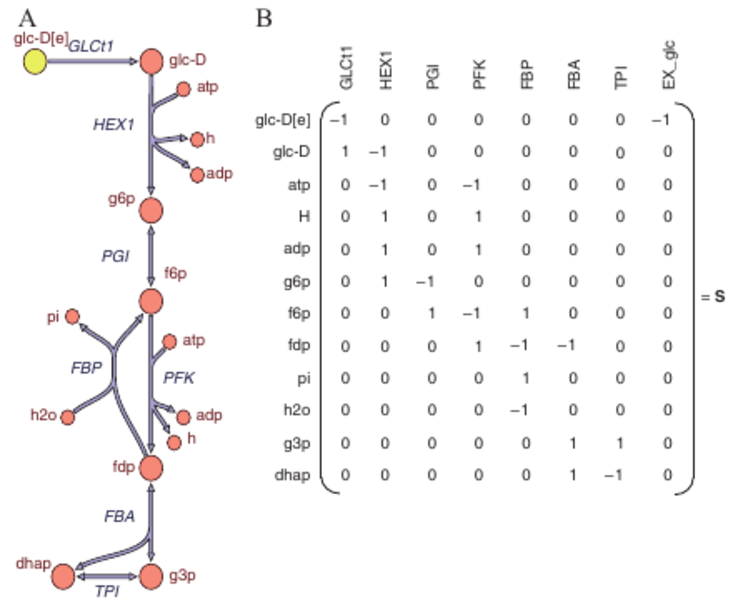
\includegraphics[width=\linewidth]{figures/Selection_011.pdf}
\caption{(create simplified version here, combine with figure \ref{fig:reconstruction_GPR_example})}
\label{fig:reconstruction_to_matrix_example}
\end{figure}

\begin{figure}[!h]
\centering
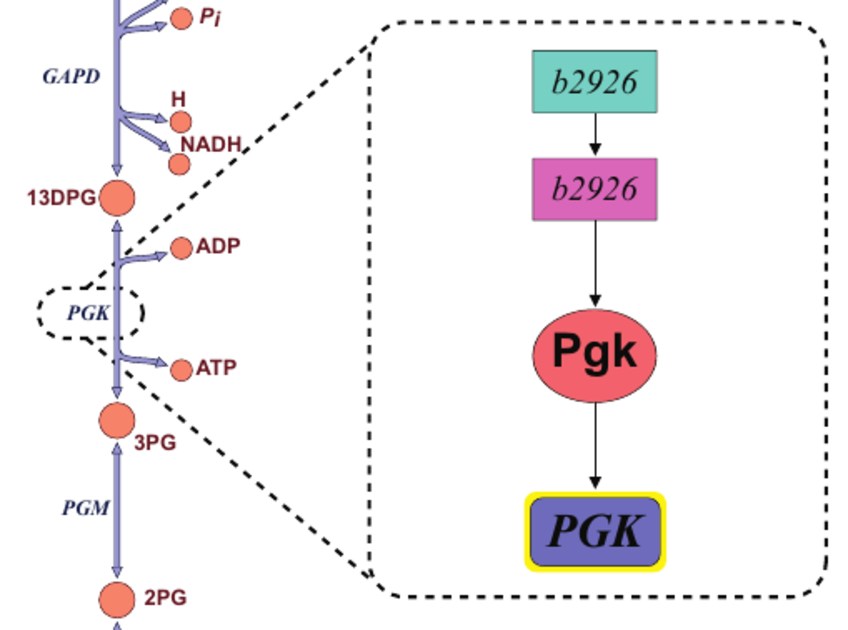
\includegraphics[width=\linewidth]{figures/Selection_013.pdf}
\caption{(create simplified version here, combine with figure \ref{fig:reconstruction_to_matrix_example})}
\label{fig:reconstruction_GPR_example}
\end{figure}

\subsection{Flux Balance Analysis}\label{ssec:flux_balance_analysis}

Flux Balance Analysis (FBA) is a mathematical tool which analysis possible flux
distributions through the metabolic network based on the stochiometric matrix of 
a GEM.

The system of linear equations built by the stoichiometric matrix $S$ of a GEM is
usually underdetermined. To choose one flux distribution from the solution space
spanned by $S$, it is assumed the organism adapted its metabolic fluxes to a certain
environment and is now in a steady state where the fluxes are optimal distributed
recording to some goal. In FBA this flux distribution is chosen by solving a
optimization problem as in equation \ref{eq:fba_optimization_formula} using linear
programming (LP) \cite{orth_what_2010}.

\begin{equation}\label{eq:fba_optimization_formula}
\begin{aligned}
& \underset{\bm{v}}{\text{max}}
& & \mu = \bm{w}^T \bm{v} \\
& \text{s.t.}
& & S\bm{v} = \bm{0}, \\
&&& \bm{v_{min}} \leq \bm{v} \leq \bm{v_{max}}
\end{aligned}
\end{equation}

The fluxes in the metabolic network $\bm{v}$ are optimized so that $\mu$ is maximized
where $\bm{w}$ is a weighting vector which defines the adaption goal of the cell.
A often used goal is to maximize the growth of the organism.
The optimization is done using mostly two constraints, (1) the stoichiometric constants $S$
for each reaction which is defined by the used GEM and (2) lower and upper bounds for 
each flux, $\bm{v_{min}}$ and $\bm{v_{max}}$, in the metabolic network but further 
constraints can be added as well.

The lower and upper bounds can be used to simulate gene know-outs by setting the upper
bound of reactions dependent on this gene to zero or to define environmental conditions
like the availability of certain metabolites.

The chosen solution by the LP solver represents a phenotype of the given organism
due to adaption to its environment but FBA has its limitations. Usually GEMs does
not model regulatory structures as activation of enzymes or regulation of gene
expressions. As the GEM does not contain kinetic parameters of the involved compounds, 
their densities can not be considered and must be modeled externally \cite{orth_what_2010}.

% \begin{itemize}
%   \item Sort introduction
%   \begin{itemize}
%     \item tool to study biochemical networks
%     \item ``calculates the flow of metabolites through
% this metabolic network''
%   \end{itemize}
%   \item What is the basic problem?
%   \begin{itemize}
%    \item stochiometric matrix can not be solved uniquely
%   \end{itemize}
%   \item How does FBA work?
%   \begin{itemize}
%     \item ``Mathematically, an
% ‘objective function’ is used to quantitatively
% define how much each reaction contributes
% to the phenotype.''
%     \item ``define a system of linear
% equations``
%     \item ''In flux balance analysis, these
% equations are solved using linear program-
% ming``
%     \item ``Every reaction can also be given
% upper and lower bounds''
%     \item ``These balances and bounds
% define the space of allowable flux distribu-
% tions of a system''
%     \item  ``To change the environmental
% conditions (such as substrate availabil-
% ity), we change the bounds on exchange
% reactions (that is, reactions representing
% metabolites flowing into and out of the sys-
% tem)``
%     \item ''Nonzero lower bounds can also
% force a minimal flux through artificial reac-
% tions [...] to sim-
% ulate energy demands not associated with
% growth``
%     \item ''Constraints can even be used to
% simulate gene knockouts by limiting reac-
% tions to zero flux''
%    \item ``Constraints are represented in two ways,
% as equations that balance reaction inputs
% and outputs and as inequalities that impose
% bounds on the system. ''
%    \item ``These stoichiometries impose
% constraints on the flow of metabolites through
% the network.''
%     \item steady state
%     
%   \end{itemize}
%   \item interpretation
%   \begin{itemize}
%     \item FBA results can be seen as phenotypes
%     \item ``FBA is an important tool for harnessing the
% knowledge encoded in these models''
%   \end{itemize}
%   \item ``FBA has limitations''
%   \begin{itemize}
%    \item ``does not use kinetic parameters, it cannot
% predict metabolite concentrations''
%     \item ``only suitable for determining fluxes at steady
% state''
%     \item `` FBA
% does not account for regulatory effects such
% as activation of enzymes by protein kinases
% or regulation of gene expression''
%   \end{itemize}
% 
% \end{itemize}



\subsection{Simulation Algorithm}

\update{
\begin{table}[h]
\centering
\caption{Overview of implemented features compared to DMMM}
\label{tab:overview_implemented_features_compared_to_dmmm}
\begin{tabular}{llllll}
\rowcolor[HTML]{EFEFEF} 
\cellcolor[HTML]{EFEFEF} Feature                  & \cellcolor[HTML]{EFEFEF}DMMM & \cellcolor[HTML]{EFEFEF}This project\\
Model                                    &   &  \\
\hspace{0.5cm}arbitrary many GEMs & yes & yes \\
\hspace{0.5cm}\begin{tabular}[c]{@{}l@{}}arbitrary many metabolites\\ in environment\end{tabular} & yes & yes \\
\hspace{0.5cm}mortablility of bacteria & \begin{tabular}[c]{@{}l@{}}yes\\(in output flux)\end{tabular} & yes \\
\hspace{0.5cm}\begin{tabular}[c]{@{}l@{}}input/output flux of bacteria\\ and metabolites\end{tabular} & yes & no \\
\hspace{0.5cm}\begin{tabular}[c]{@{}l@{}}parameterized initial state\\ of environment composition\end{tabular} & yes & yes \\
\hspace{0.5cm}Michaelis-Menten kinetics & yes & yes \\
Algorithm &  &  \\
\hspace{0.5cm}ODE solver & yes & yes \\
\hspace{0.5cm}different ODE solvers & yes & no \\
\hspace{0.5cm}analytical solver & yes &no \\
\end{tabular}
\end{table}}

As described by Zhuang et al. in \cite{zhuang_genome-scale_2011} the algorithm uses an ODE solver with embedded FBA. An FBA is solved
for each GEM in the model and for each time step in the discretised simulation time interval considering the changed metabolite and
bacteria densities in the shared environment. The results of the FBAs are used by the ODE solver to solve the differential equations

\update{
\begin{equation} \label{eq:diff_eq_x}
	\frac{\dd x_j}{\dd t} = (v_{v_\bio} - \mu(v_{\bio}) x_j
\end{equation}
\begin{equation} \label{eq:diff_eq_s}
	\frac{\dd s_i}{\dd t} = \displaystyle\sum_{j=1}^{N} v_{i,j} x_j
\end{equation}

\update{
which models the dynamics of the bacteria's environment \cite{zhuang_design_2012} where $i = 1,\dotsc,N$ is the index of metabolites in the shared environment and $j = 1,\dotsc,M$ is the index of bacteria.
The bacteria density is modeled in $x_j$ with $\left[ x_j \right] = \si{\gram}$ and $\mu_j$ is the bacteria's growth rate with $[\mu_j] = \si{\gram\per\gram_{DW}\per\hour}$\footnote{$\si{\gram_{DW}}$ stands for grams dry weight, i.e. grams of bacteria after all water has evaporated}.
Input and output fluxes of the bacteria's models are modeled in $v_{i,j}$ with $\left[ v_{i,j} \right] = \si{\milli\mole\per\gram_{DW}\per\hour}$,
the densities of metabolites in the shared environment in $s_i$ with $\left[ s_i \right] = \si{\milli\mole\per\liter}$.}

In each time step each bacteria's metabolite intake must be changed dependent on the densities of the metabolites in the shared environment.
To model saturation of metabolite intake for high metabolite densities Zhuang et al. implemented Michaelis-Menten kinetics \cite{johnson2011original}

\begin{equation} \label{eq:michaelis-menten}
% b_{M,m} = \frac{v_{max,M,m} s_m}{s_m + k_{M,m}} \prod_{a=1}^M \frac{1}{1 + \frac{s_a}{\mat{I}_{a,i,j}}}
 b_{M,m} = v_{max,M,m} \; \frac{s_m}{k_{M,m}+s_m} \; \prod_{m'} \cfrac{1}{1+\cfrac{s_{m'}}{\mat{I}_{M,m,m'}}}
\end{equation}

This formula describes the upper bound of the input flux $b_{M,m}$ for metabolite m of model M dependent on the metabolite density
$s_m$. The formula is characterized by two constants $\left[ v_{max,M,m} \right] = \si{\milli\mole\per\gram_{DW}\per\hour}$ and $\left[ k_{M,m} \right] = \si{\milli\mole\per\liter}$
for each bacteria and metabolite. $s_{m'}$ is the metabolite density of metabolite $m'$, $\mat{I}_{M,m,m'}$ is the inhibition constant of metabolite $m'$ and
describes the inhibition of the intake of metabolite $m$ by metabolite $m'$ at model $M$.

Mortality is considered using a function $\mu_M(v_\bio)$ $\left[ \mu_{M} \right] = \si{\milli\mole\per\gram_{DW}\per\hour}$ for each organism $M$ in this implementation while Zhuang et al. modeled this
using the output flux of bacteria out of the system.
Yeast cells have a mean lifetime of 26 cell divisions, making the mortality dependant on the biomass production $v_\bio$.
We have a doubling rate of $t_d=\frac{\log(2)}{b}$, i.e. every cell doubles every $t_d$ hours. Hence, cells have a lifetime of $t_l=26\mul t_d$ hours.
Consider a population of $N$ cells, which have been born equidistantly. On average, $\frac{N}{t}$ cells die every hour.
The populations mortality is therefore $\frac{N}{t} \mul \frac{1}{N}=\frac{1}{t_l}=\frac{b}{26\mul \log(2)}$

Algorithm \ref{alg:differential_equation_with_embedded_fba} shows a basic implementation of the differential equations solved by an ODE
solver during the simulation similar to DMMM \cite{zhuang_genome-scale_2011}.

\update{
The algorithm expects a list of bacteria models consisting of
\begin{itemize}
 \item GEM of this bacteria: A, $\bm{v_{min}}$, $\bm{v_{max}}$, $\bm{w_{growth}}$
 \item $\bm{v_{mm}}$ (Michaelis-Menten $V_{max}$) for each exchange metabolite and species
 \item $\bm{k}$ (Michaelis-Menten K) for each exchange metabolite and species
 \item mortality $\mu(v_\bio)$
 \item inhibition constants $\mat{I}_a$
\end{itemize}}

Furthermore a list of all exchange metabolites in the environment, the bacteria and metabolite densities.


\begin{algorithm}
	\DontPrintSemicolon
	\def\model{\ensuremath{\mathrm{model}}}
    \KwIn{bacteria populations $x_j$, metabolite counts $S_i$}
    \KwOut{slope of bacteria and metabolite densities $\dot{x}_j, \dot{s}_i$}
    \KwData{bacteria models $\model_j$, Michaelis-Menten constants of model $M$ $\v{k}_{M}$, inhibition matrices of model $M$  $\mat{I}_{M}$, Total volume $V$}
    
    $s_i \KwAssign \frac{S_i}{V}$\;
    
    $S_{<0} \KwAssign \{m | S_m < 0\}$\;
    $x_{<0} \KwAssign \{j | x_j < 0\}$\;

    
	$\v s(S_{<0}) = 0$\;
	$\v x(S_{<0}) = 0$\;
	
	\ForEach{model $M$ in models}{
		\ForEach{metabolite $m$ in exchanges of $M$}{
%			$\displaystyle b_{M,m} = v_{max,M,m} \; \frac{s_m}{k_{M,m}+s_m} \; \prod_{m'} \cfrac{1}{1+\cfrac{s_{m'}}{\mat{I}_{M,m,m'}}}$\;
			$b_{M,m} = \mathrm {upper\_bound}(\v{s}, M, m)$
		}
	}
	
	$\dot{\v x} \KwAssign [0,\dotsc,0]$\;
	$\dot{\v S} \KwAssign [0,\dotsc,0]$\;
	
    \ForEach{Model $M$ in models}{
      $v_\bio, \bm{v}$ \KwAssign $\mathrm {FBA}(M)$\;
      $\dot{x}_M = (\bio - \mu(v_bio)) \mul x_M$\;
      $\dot{\v S} = \dot{\v S} + \v v \mul x_M$\;
    }
    
	$\dot{\v S}(S_{<0}) = \max\{0,\dot{\v S}(S_{<0})\}$\;    
	$\dot{\v x}(x_{<0}) = \max\{0,\dot{\v x}(x_{<0})\}$\;    
    
    \Return{$[\dot{\v x},\dot{\v S}]$}
    \caption{Differential equation with embedded FBA}
    \label{alg:differential_equation_with_embedded_fba}
\end{algorithm}

In a first step, the absolute metabolite counts are converted to densities, and all smaller than zero entries are set to zero. This step is necessary since negative densities are unphysical and forbidden, hence the function is transformed as proposed in \cite{shampine_nonneg_2005}.

Next, the lower bounds of the intake fluxes are updated for each bacteria $M$ and exchange metabolite $m$ according to the Michaelis-Menten formula \ref{eq:michaelis-menten}.

\update{
In a further step, the GEMs are optimized for growth using FBA, the results are used as biomass production $\bm{v}_\bio$ and actual input and output
fluxes $\bm{v_j}$ of bacteria j in this time step.
The mortality is considered by subtracting the constants $\bm{\mu(\v{v}_\bio}$ from the biomass production rates $\bm{v}_\bio$.
The slopes $\dot{\bm{x}}$ and $\bm{\dot{s}}$ are calculated according to \ref{eq:diff_eq_x} and \ref{eq:diff_eq_s} and, if any of the populations or metabolites were negative, their derivatives are cut-off to be always larger than 0.}

\subsection{Simulation Setup}\label{ssec:simulation_setup}

The goal of the simulation is to validate the basic functionality of the simulator using a simplified setup of a realistic future
simulation scenario. As defined in the project goals, this simulation scenario is the dynamic flux balance analysis (DFBA) of a
co-culture of Saccharomyces cerevisiae and Lactobacillus plantarum.

\update{
As genome-scale models a model of Lactobacillus plantarum published by Teusink et al. \cite{teusink_analysis_2006}. A decision about
a yeast model is not made yet.}

\update{
The simulation will consider two main input metabolites: oxygen and glucose. Table \ref{tab:model_constants_simulation_setup} and table
\ref{tab:simulation_parameters_simulation_setup} contain all values needed to define the initial metabolite conditions and kinetics.}

\update{
\begin{table}[h]
\centering
\caption{Model constants used in the simulation setup}
\label{tab:model_constants_simulation_setup}
\begin{tabular}{llllll}
\rowcolor[HTML]{EFEFEF} 
\cellcolor[HTML]{EFEFEF} Constant          & \cellcolor[HTML]{EFEFEF}S. cerevisiae & \cellcolor[HTML]{EFEFEF}L. plantarum\\
Maximum glucose uptake rate (mmol/g/h)     & 18.5 & 18.5 \\
Maximum oxygen uptake rate (mmol/g/h)      & 2.5 & 2.5 \\
Glucose uptake saturation constant (g/l)   & 0.5 & 0.5 \\
Oxygen uptake saturation constant (mmol/l)     & 0.005 & 0.005 \\
Mortability (?)                            & ? & ? \\
Glucose uptake inhibition by ethanol constant (g/l)     & 10\cite{hjersted_genome-scale_2007} & - \\
Glucose uptake inhibition by lactic acid constant (mol/mol ?)     & TBD & - \\
\end{tabular}
\end{table}}

% E-Mail from Steinn about model constants of L. plantarum from 12.04.2018:
% ----------------------------------------------------------------------------------------------
% As a first approximation I would assume the same v_max and k_m for L. plantarum as in yeast.
% 
% The maximum glucose uptake rate can be assumed to be similar to yeast for the time being 
% (for Lactobacillus reuteri it is approx. 21 mmol/gDW/h [gDW = grams dry weight]). L. plantarum 
% is an anaerobe that can tolerate oxygen (and has some oxygen dependent metabolism as well) but
% as a first approximation I would assume that oxygen plays a minor role, hence the oxygen
% saturation constant may not be too important.
% ----------------------------------------------------------------------------------------------
\update{
\begin{table}[h]
\centering
\caption{Simulation parameters used in the simulation setup}
\label{tab:simulation_parameters_simulation_setup}
\begin{tabular}{llllll}
\rowcolor[HTML]{EFEFEF} 
\cellcolor[HTML]{EFEFEF} Parameter          & \cellcolor[HTML]{EFEFEF}value & \cellcolor[HTML]{EFEFEF}reference\\
Initial glucose density (mmol/l) & 272.9 ... 1230.755 & equation \ref{eq:ready_to_use_plato_to_metabolite_density}, table \ref{tab:constants_used_in_this_document} \\
Initial oxygen density (mmol/l)  & 0.5039 & equation \ref{eq:init_oxygen_density}, table \ref{tab:constants_used_in_this_document}\\
Initial density of S. cerevisiae (mmol/l) & ? & - \\
Initial density of L. plantarum (mmol/l) & ? & - \\
\end{tabular}
\end{table}}

\update{
To verify the basic functionality of the simulator the resulting bacteria densities and metabolite densities of ethanol, d- and l-lactate,
oxygen and glucose will be compared to existing data.}

\subsection{Software Stack}
	This DFBA simulator framework uses Python version 3 as programming language and builds on the CobraPy Framework \cite{ebrahim_cobrapy_2013}.
	As solver for the linear programs during the FBA the GNU Linear Programming Kit (GLPK) is used.
	To integrate the ODEs, the Python package scipy.integrate.ode is used, employing the dopri5 solver, which is a classical Runge-Kutta explicite ODE solver for non-stiff problems \cite{hairer1993solving}.


\section{Results}\label{sec:results}
	At a first stage, yeast and lactic bacteria monocultures were simulated to verify whether they work independantly of each other.
	At the second stage, the coculture was simulated to show.
	
	The mediums used contain \SI{50}{\litre} of water mixed with an inital glucose concentration of \SI{1000}{\milli\mole\per\litre}.
	\subsection{Yeast Monoculture}\label{ssec:yeast_monoculture}
		The yeast monocolture is well-behaved, until the very edges of metabolic activity, where the GEM is blocked.
		But its growth is almost exponential, as can be seen in Figure \ref{fig:yeast_0lac_pop}.
		The steep curve at the beginning marks the region where oxygen can be metabolised.
		The slight curvature of the following section can be explained by the self-inhibition of the organism,
		caused by the toxicity of ethanol, and by the sinking glucose concentration.
		Concentrations of the relevant metabolites that can be seen in Figure \ref{fig:yeast_0lac_met}.
		
		At time $t\approx 25$ the GEM is blocked since the glucose uptake can not satisfy the ATP maintenance reactions anymore;
		the population starts to die.
		\begin{figure}[h]
			\centering
			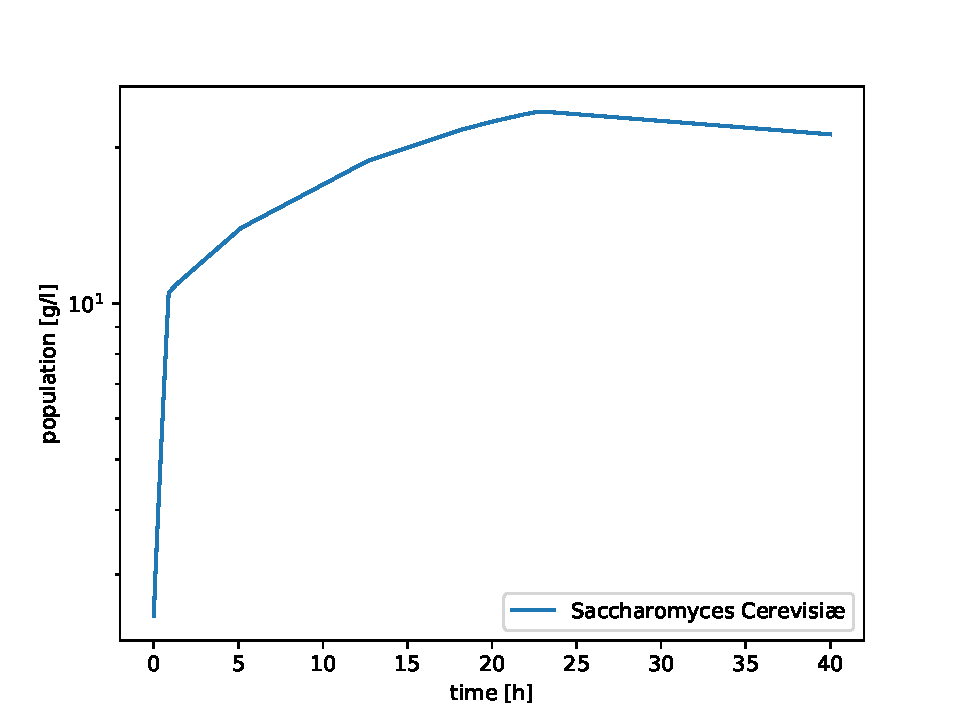
\includegraphics[width=\linewidth]{figures/results/yeast/0lac_populations.pdf}
			\caption{The yeast growth in the medium in a logarithmic scale}
			\label{fig:yeast_0lac_pop}
		\end{figure}
		\begin{figure}[h]
			\centering
			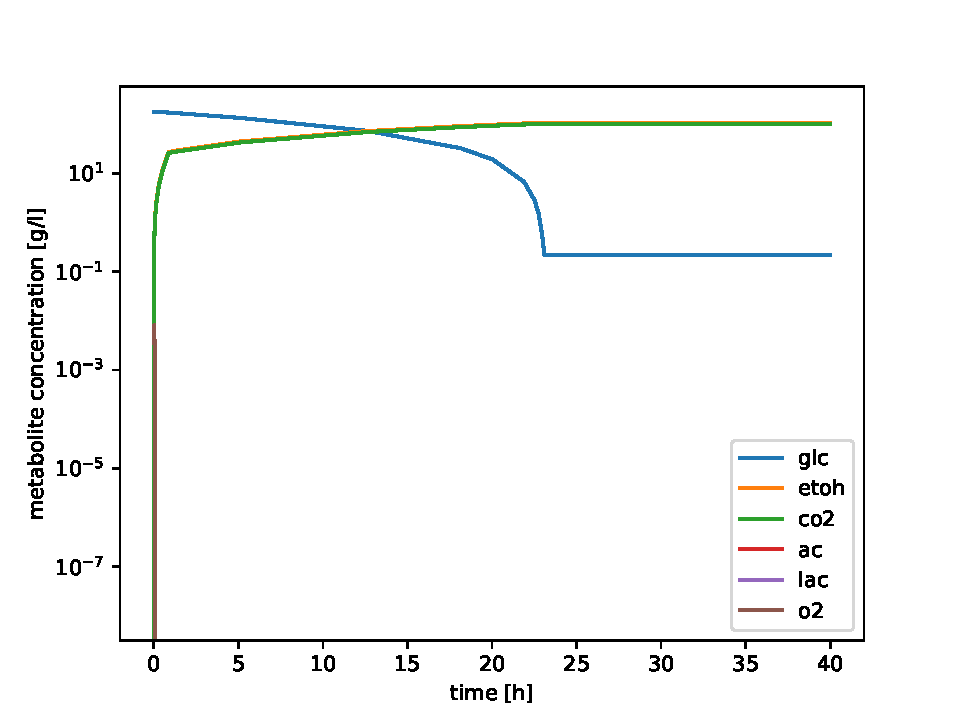
\includegraphics[width=\linewidth]{figures/results/yeast/0lac_metabolites.pdf}
			\caption{The concentrations of interesting metabolites in the simulated medium for yeast monocultures}
			\label{fig:yeast_0lac_met}
		\end{figure}
		
		In further simulations the concentration of lactate was increased, and the toxicity of the lactate was tuned to best fit the curves given in Figure \ref{fig:yeast_real}.
		This was achieved with a number of $I_{Y,\mathrm{glc,lac}}=\SI{30}{\milli\mole\per\litre}$. Figure \ref{fig:yeast_simfig} shows the tuned curves.
		
		The fit is not perfect on multiple accounts: Firstly, the organism takes longer to metabolise the glucose, which can be traced back to a too high ethanol inhibition constant $I_{Y,\mathrm{glc,etoh}}$
		Secondly, there are sharp, seemingly non-smooth corners in the plot. These can be explained by wrong Michaelis-Menten constants $k_{Y,m}$
		
		Adapting these constants to $k_{Y,\mathrm{glc}}=\SI{15}{\milli\mole\per\litre}$ and the inhibition constant to $I_{Y,\mathrm{glc,etoh}}=\SI{350}{\gram\per\liter}$ yields a better fitting result
		shown in Figure \ref{fig:yeast_better_simfig}
		
		For the remainder of the simulations, the constants were reset to the original values.
		
		\begin{figure}[h]
			\centering
			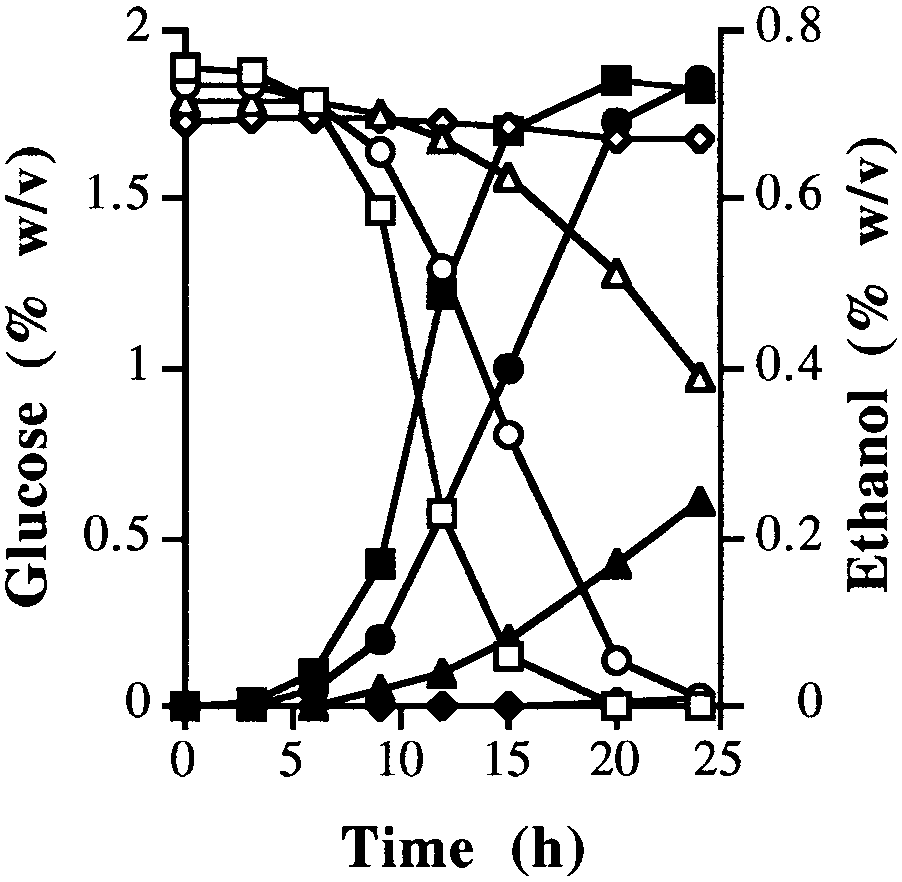
\includegraphics[width=0.6\linewidth]{figures/yeast_real.png}
			\caption{Glucose and ethanol concentrations measured in a real-life scenario with varying lactate concentrations \cite{Narendranath2001}. }
			\label{fig:yeast_real}
		\end{figure}
		
		\begin{figure}[h]
			\centering
			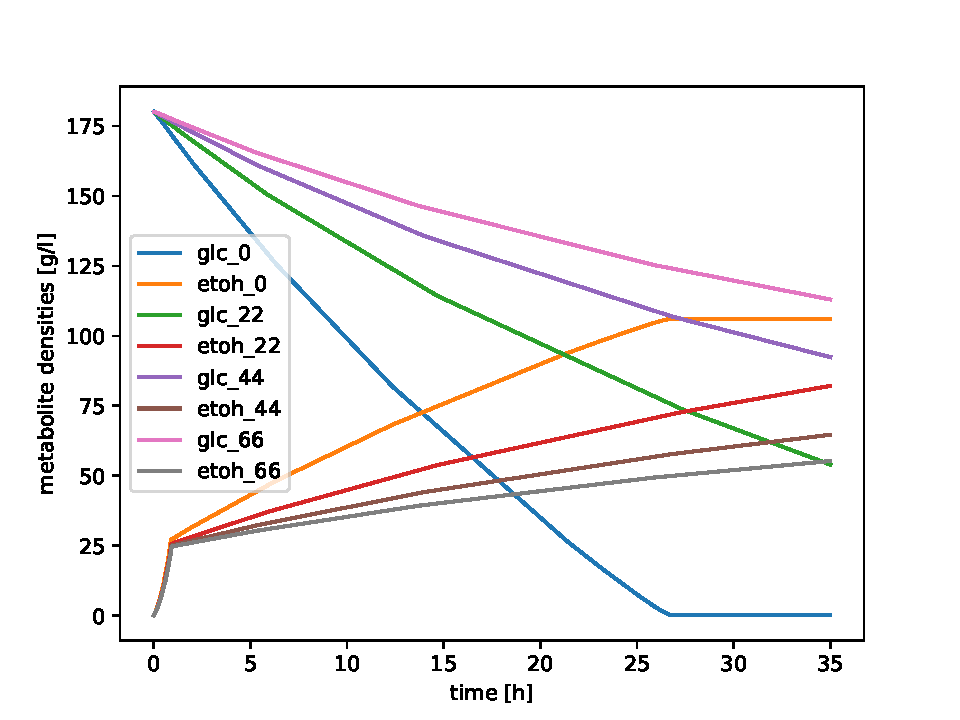
\includegraphics[width=\linewidth]{figures/results/yeast/similar_plot.pdf}
			\caption{The ethanol and glucose concentration at different concentrations of lactate}
			\label{fig:yeast_simfig}
		\end{figure}

		\begin{figure}[h]
			\centering
			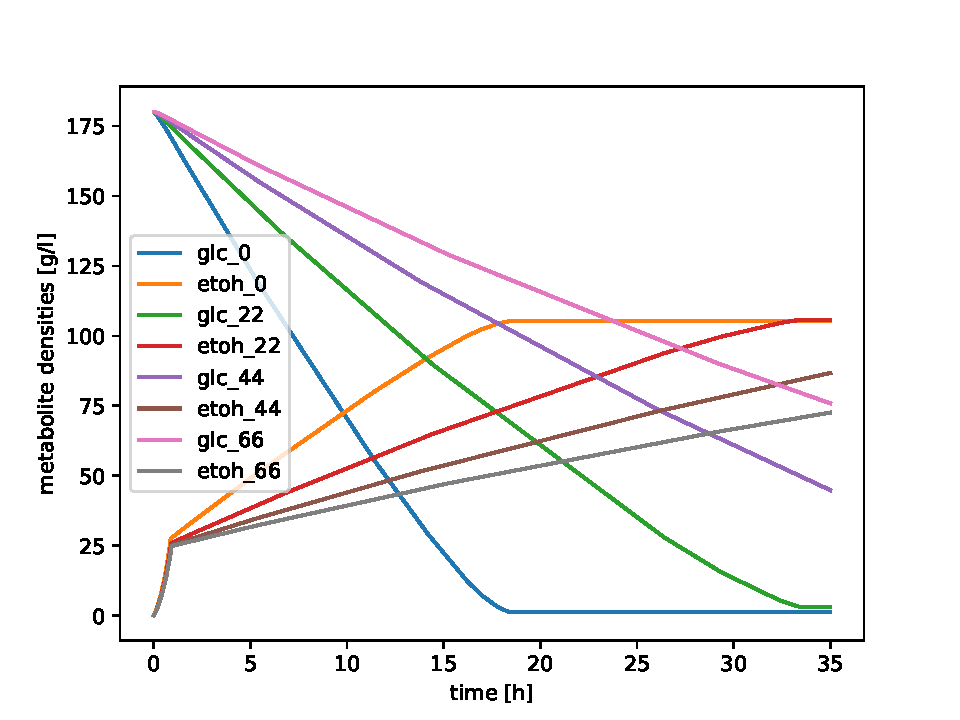
\includegraphics[width=\linewidth]{figures/results/better_yeast/similar_plot.pdf}
			\caption{The ethanol and glucose concentration at different concentrations of lactate with the improved constants}
			\label{fig:yeast_better_simfig}
		\end{figure}
		
	\subsection{Lactobacillus Plantarum}
		If we add Lactobacillus Plantarum to the same medium without the yeast, we get the population curves in Figure \ref{fig:lb_pop}.
		These, too, are what can be expected (i.e. exponential growth that gets dampened as the glucose runs out and ad the environment becomes more toxic).
		
		An interesting side-effect of the Lactobacilli is that they not only produce lactate and acetate, but also a rather large amount of ethanol.
		\begin{figure}[h]
			\centering
			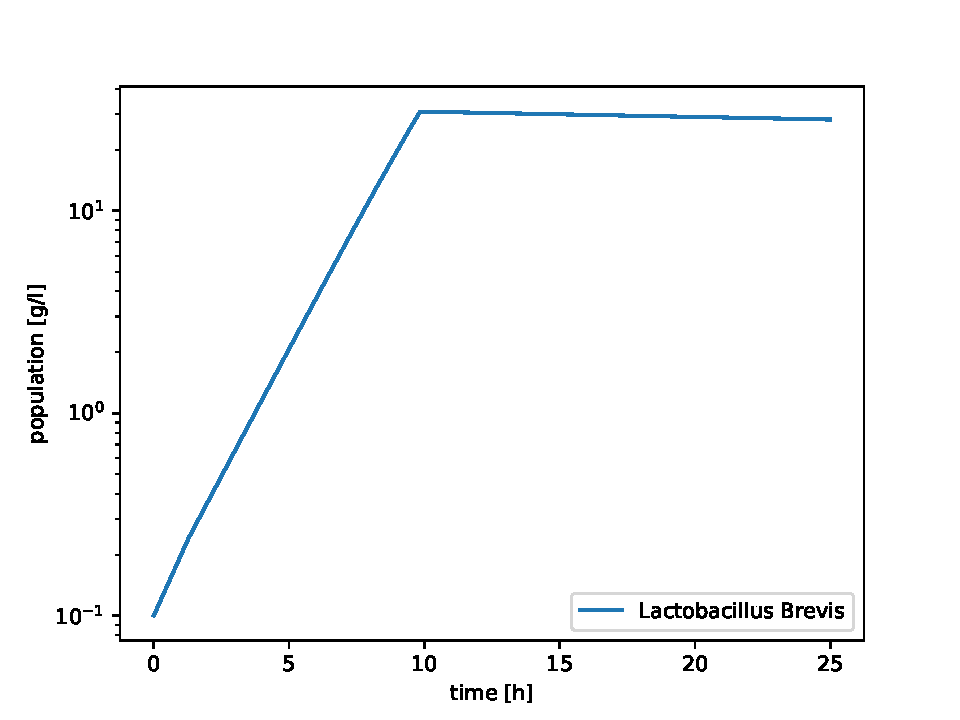
\includegraphics[width=\linewidth]{figures/results/lactobacillus/lactobacillus_populations.pdf}
			\caption{The growth of Lactobacillus Plantarum in the medium in a logarithmic scale}
			\label{fig:lb_pop}
		\end{figure}
		
		\begin{figure}[h]
			\centering
			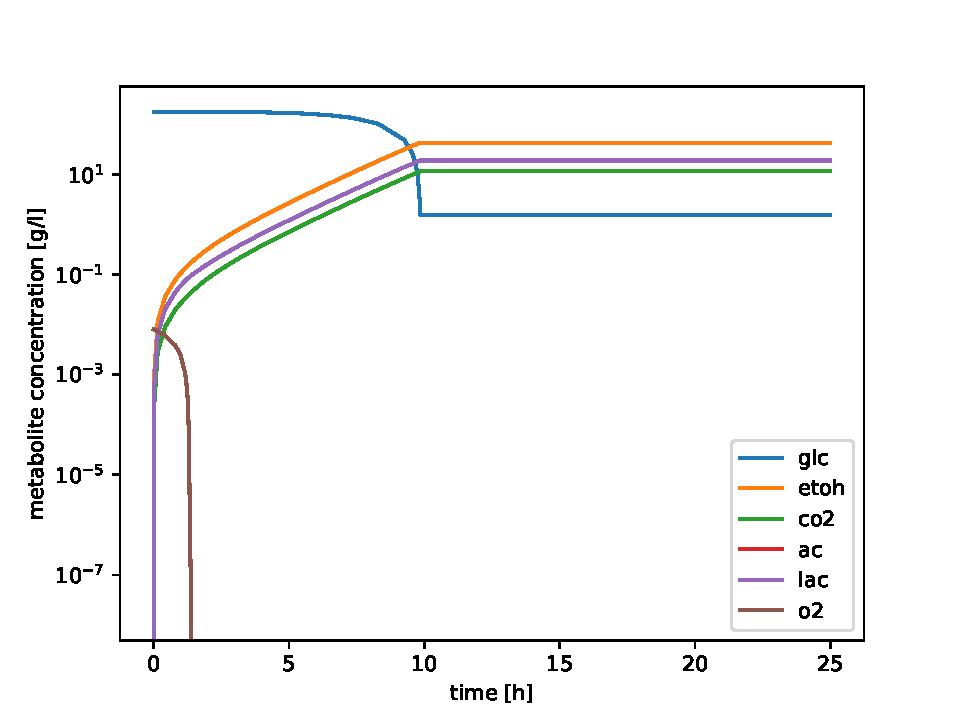
\includegraphics[width=\linewidth]{figures/results/lactobacillus/lactobacillus_metabolites.pdf}
			\caption{The concentrations of interesting metabolites in the simulated medium for Lactobacillus Plantarum monocultures}
			\label{fig:lb_met}
		\end{figure}
	
	\subsection{Cocultures}
		The simulation of the cocultures shows many effects known by experiment.
		The yeast shows much higher activity relative to the lactic bacteria when the medium contains oxygen, as can be seen in both Figure \ref{fig:cocult_0.1_met} and \ref{fig:cocult_1_met}.
		This is congruent with the common brewing practice of aerating the wort before actually fermenting it \cite[P. 168]{daniels1996designing}.
		More oxygen gives the yeast an additional head start in population.
		
		Additionally, whether the Lactobacilli overtake the yeast is dependant on the initial concentration of Lactobacillus Plantarum.
		This can be seen in Figure \ref{fig:cocult_pops}.
		
		\begin{figure}[h]
			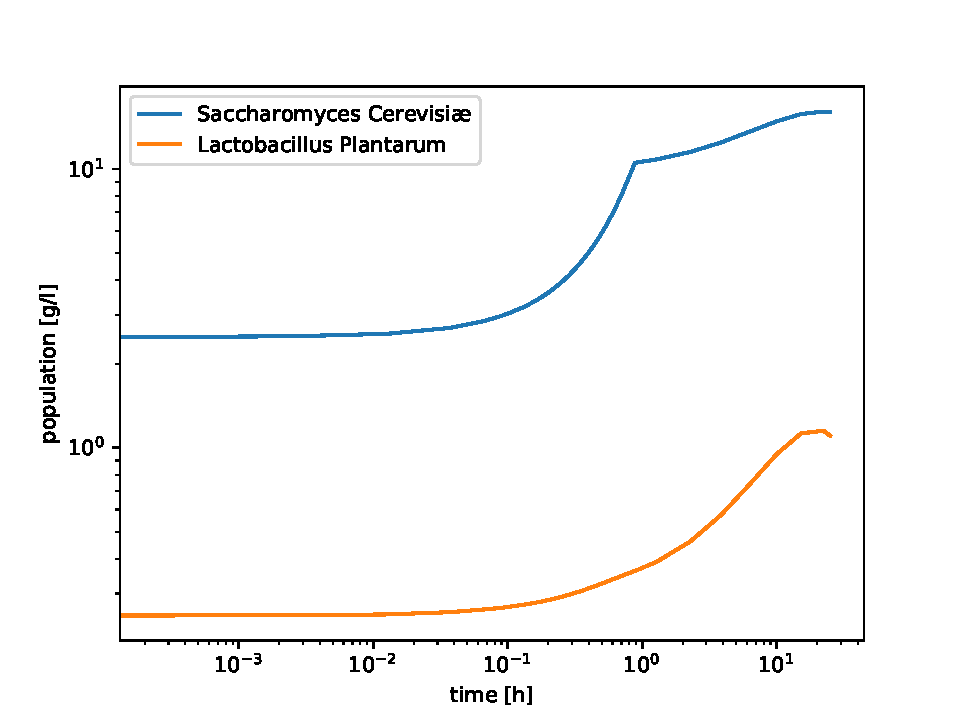
\includegraphics[width=\linewidth]{figures/results/cocultures/0_1_populations.pdf}
			\caption{The population of the two organisms with \SI{0.05}{\gram\per\litre} initial lactobacillus population}
			\label{fig:cocult_0.1_pop}
		\end{figure}
		
		\begin{figure}[h]
			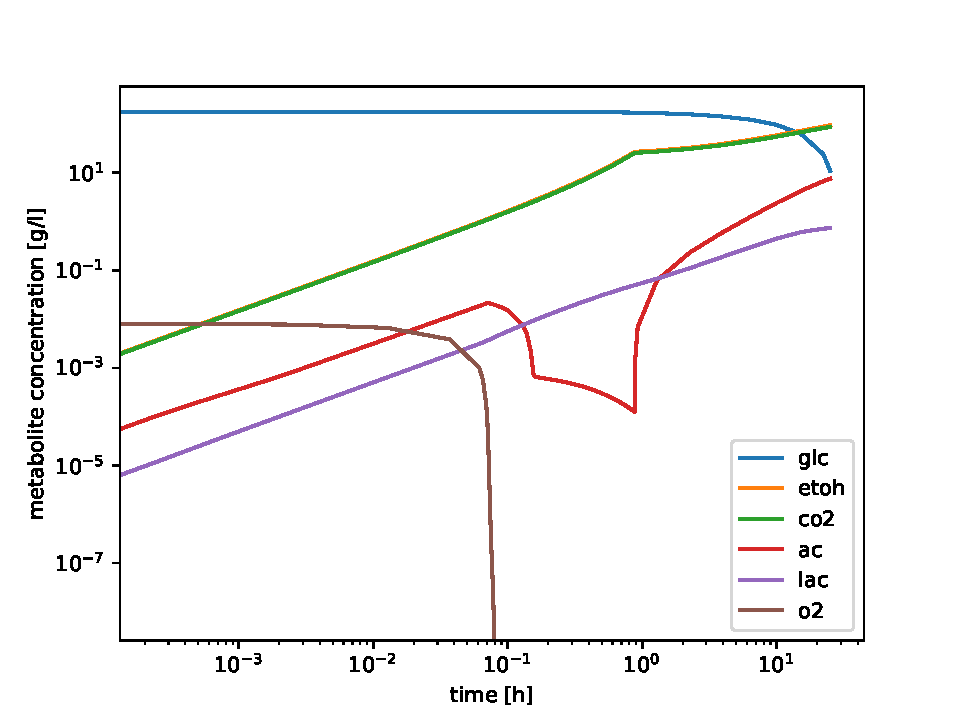
\includegraphics[width=\linewidth]{figures/results/cocultures/0_1_metabolites.pdf}
			\caption{The metabolites in the medium with \SI{0.05}{\gram\per\litre} initial lactobacillus population}
			\label{fig:cocult_0.1_met}
		\end{figure}
		
		\begin{figure}[h]
			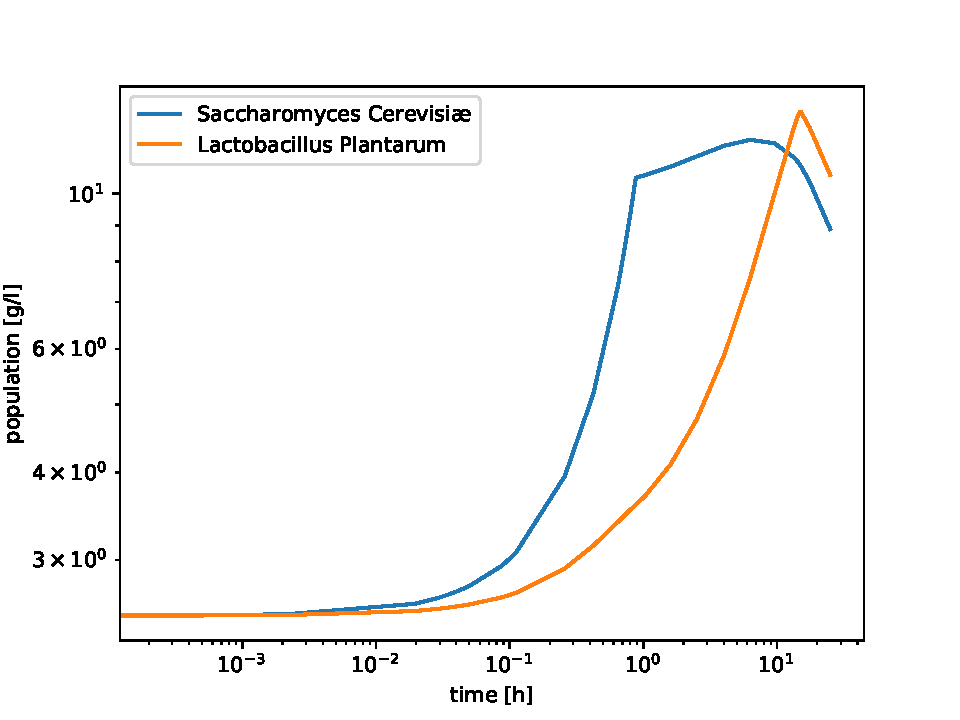
\includegraphics[width=\linewidth]{figures/results/cocultures/1_populations.pdf}
			\caption{The population of the two organisms with \SI{0.5}{\gram\per\litre} initial lactobacillus population}
			\label{fig:cocult_1_pop}
		\end{figure}
		
		\begin{figure}[h]
			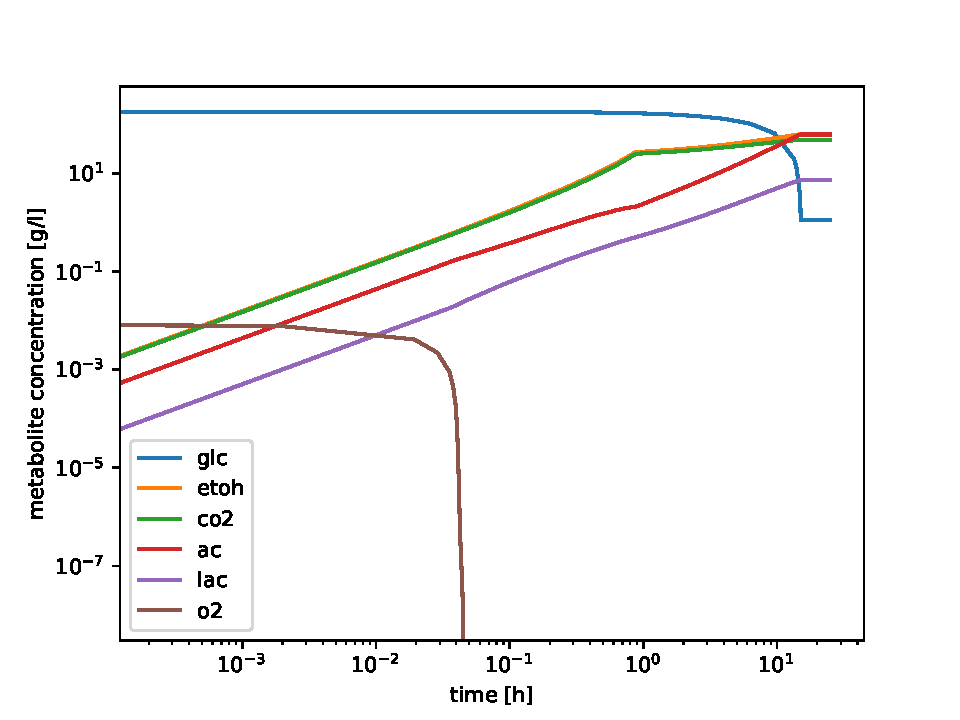
\includegraphics[width=\linewidth]{figures/results/cocultures/1_metabolites.pdf}
			\caption{The metabolites in the medium with \SI{0.5}{\gram\per\litre} initial lactobacillus population}
			\label{fig:cocult_1_met}
		\end{figure}
		
		\begin{figure}[h]
			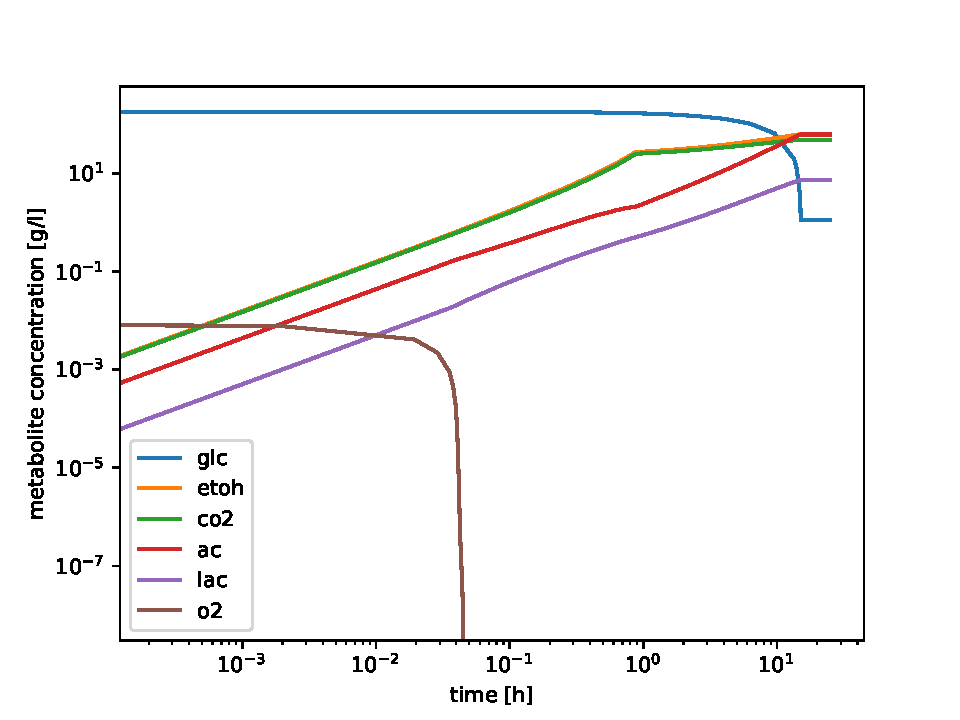
\includegraphics[width=\linewidth]{figures/results/cocultures/1_metabolites.pdf}
			\caption{The populations over multiple initial Lactobacillus concentrations (0.05, 0.5, 5, 50)}
			\label{fig:cocult_pops}
		\end{figure}


\section{Conclusions}\label{sec:conclusions}




% An example of a floating figure using the graphicx package.
% Note that \label must occur AFTER (or within) \caption.
% For figures, \caption should occur after the \includegraphics.
% Note that IEEEtran v1.7 and later has special internal code that
% is designed to preserve the operation of \label within \caption
% even when the captionsoff option is in effect. However, because
% of issues like this, it may be the safest practice to put all your
% \label just after \caption rather than within \caption{}.
%
% Reminder: the "draftcls" or "draftclsnofoot", not "draft", class
% option should be used if it is desired that the figures are to be
% displayed while in draft mode.
%
%\begin{figure}[!t]
%\centering
%\includegraphics[width=2.5in]{myfigure}
% where an .eps filename suffix will be assumed under latex, 
% and a .pdf suffix will be assumed for pdflatex; or what has been declared
% via \DeclareGraphicsExtensions.
%\caption{Simulation Results}
%\label{fig_sim}
%\end{figure}

% Note that IEEE typically puts floats only at the top, even when this
% results in a large percentage of a column being occupied by floats.


% An example of a double column floating figure using two subfigures.
% (The subfig.sty package must be loaded for this to work.)
% The subfigure \label commands are set within each subfloat command, the
% \label for the overall figure must come after \caption.
% \hfil must be used as a separator to get equal spacing.
% The subfigure.sty package works much the same way, except \subfigure is
% used instead of \subfloat.
%
%\begin{figure*}[!t]
%\centerline{\subfloat[Case I]\includegraphics[width=2.5in]{subfigcase1}%
%\label{fig_first_case}}
%\hfil
%\subfloat[Case II]{\includegraphics[width=2.5in]{subfigcase2}%
%\label{fig_second_case}}}
%\caption{Simulation results}
%\label{fig_sim}
%\end{figure*}
%
% Note that often IEEE papers with subfigures do not employ subfigure
% captions (using the optional argument to \subfloat), but instead will
% reference/describe all of them (a), (b), etc., within the main caption.


% An example of a floating table. Note that, for IEEE style tables, the 
% \caption command should come BEFORE the table. Table text will default to
% \footnotesize as IEEE normally uses this smaller font for tables.
% The \label must come after \caption as always.
%
%\begin{table}[!t]
%% increase table row spacing, adjust to taste
%\renewcommand{\arraystretch}{1.3}
% if using array.sty, it might be a good idea to tweak the value of
% \extrarowheight as needed to properly center the text within the cells
%\caption{An Example of a Table}
%\label{table_example}
%\centering
%% Some packages, such as MDW tools, offer better commands for making tables
%% than the plain LaTeX2e tabular which is used here.
%\begin{tabular}{|c||c|}
%\hline
%One & Two\\
%\hline
%Three & Four\\
%\hline
%\end{tabular}
%\end{table}


% Note that IEEE does not put floats in the very first column - or typically
% anywhere on the first page for that matter. Also, in-text middle ("here")
% positioning is not used. Most IEEE journals use top floats exclusively.
% Note that, LaTeX2e, unlike IEEE journals, places footnotes above bottom
% floats. This can be corrected via the \fnbelowfloat command of the
% stfloats package.





% if have a single appendix:
%\appendix[Proof of the Zonklar Equations]
% or
%\appendix  % for no appendix heading
% do not use \section anymore after \appendix, only \section*
% is possibly needed

% use appendices with more than one appendix
% then use \section to start each appendix
% you must declare a \section before using any
% \subsection or using \label (\appendices by itself
% starts a section numbered zero.)
%


\appendices
\section{}\label{ap:super_fancy_stuff}
The following approximation is used to convert \textdegree P (``degree plato'') to a density measure (\si{\gram\per\liter})\cite{bubnik1995sugar}.
\begin{equation} \label{eq:grad_plato_to_density}
 d_{total} = 4.13 \frac{g}{l \,\,\, ^\circ P} p + 997 \frac{g}{l}
\end{equation}

As the simulation framework expects metabolite densities relative to the total volume of the solution (mmol of metabolite per liter
solution, mmol/l) the total density $d_{total}$ must to converted to a density $s_{glc}$.
It is assumed that $V_{total} = V_{glc} + V_W$. Furthermore $m$ is used in the following equations as a measure of mass.

\begin{align}\label{eq:total_density_to_metabolite_density}
 d_{total} & = \frac{m_{total}}{V_{total}} \nonumber \\
           & = \frac{m_{glc} + m_w}{V_{total}} \nonumber \\
           & = \frac{m_{glc} + d_w V_w}{V_{total}} \nonumber \\
           & = \frac{m_{glc} + d_w \left(V_{total} - V_{glc}\right)}{V_{total}} \nonumber \\
           & = \frac{m_{glc} + d_w \left(V_{total} - \frac{m_{glc}}{d_{glc}}\right)}{V_{total}} \nonumber \\
 \Leftrightarrow \quad s_{glc}   & = \frac{m_{glc}}{V_{total}} = \frac{d_{total} - d_w}{1 - \frac{d_w}{d_{glc}}}
\end{align}

Combining equation \ref{eq:grad_plato_to_density} and \ref{eq:total_density_to_metabolite_density}, including all constants and converting it to mmol/l leads to:
\begin{equation} \label{eq:ready_to_use_plato_to_metabolite_density}
 s_{glc} = \left( 63.857 \frac{1}{^\circ P} p - 46.385 \right) \frac{mmol}{l}
\end{equation}




\begin{table}[h]
\centering
\caption{Constants used in this document}
\label{tab:constants_used_in_this_document}
\begin{tabular}{llllll}
\rowcolor[HTML]{EFEFEF} 
\cellcolor[HTML]{EFEFEF} Constant    & \cellcolor[HTML]{EFEFEF}symbol      & \cellcolor[HTML]{EFEFEF}value & \cellcolor[HTML]{EFEFEF}reference\\
Oxygen saturation of water at 20\textdegree C (mg/l) & -  & 9.077 & \cite{fao_water_1987} \\
Molar mass of water (g/mol)    & -   & 18.015 & \cite{pupchen_website}\\
Molar mass of glucose (g/mol) & -  & 180.156 & \cite{pupchen_website}\\
Density of water (g/l) & $d_w$ & 1.00 &  \cite{pupchen_website}\\
Density of glucose (g/l) & $d_{glc}$ &  1.56 & \cite{pupchen_website}\\
Typical glucose/water solution density to brew beer (\textdegree P) & - & 5...20 & - \\
\end{tabular}
\end{table}

To calculate the initial oxygen density in the solution it is assumed that the solution is at 20 \textdegree C and fully saturated
with oxygen:
\begin{equation} \label{eq:init_oxygen_density}
s_{init,ox} = 9.077 \frac{mg}{l} = 9.077 \,\, 10^{-3}  \frac{g}{l} = \frac{9.077 \,\, 10^{-3} \frac{g}{l}}{18.015 \,\, 10^{-3} \frac{g}{mmol}} = 0,5039 \frac{mmol}{l} 
\end{equation}

% you can choose not to have a title for an appendix
% if you want by leaving the argument blank
\section{}\label{ap:more_super_fancy_stuff}
\begin{table}[]
\centering
\caption{Rating of considered DFBA methods}
\label{tab:rating_of_DFBA_methods}
\begin{tabular}{llll}
\rowcolor[HTML]{EFEFEF} 
Method                                                                                                 & \begin{tabular}[c]{@{}l@{}}comp.\\ effort\end{tabular} & \begin{tabular}[c]{@{}l@{}}impl.\\ complexity\end{tabular} & flexibility \\
dynamic optimization approach (DOA)                                                                    & high                                                   & medium-high                                                & ?           \\
static optimization approach (SOA)                                                                     & low                                                    & low                                                        & low         \\
direct approach (DA)                                                                                   & medium                                                 & low                                                        & medium      \\
\begin{tabular}[c]{@{}l@{}}reformulation to a differential-glgebraic\\ equation system\end{tabular} & low-medium                                             & high                                                       & ?          
\end{tabular}
\end{table}

\section{}
\begin{table}[]
\centering
\caption{Variables, constants and their units}
\label{tab:units_of_variables_and_constants}
\begin{tabular}{lll}
\rowcolor[HTML]{EFEFEF} 
Symbol                 & Unit    & Description\\
$M$                    & -       & bacteria model\\
$m$                    & -       & metabolite in shared medium\\
$X_M$                  & \si{\gram_{DW}} & dry weight of bacteria $M$ in shared medium\\
$v_{M,m}$              & \si{\milli\mole\per\gram_{DW}\per\hour} & input/output flux of model $M$\\
$\mu_M$                & \si{\gram\per\gram_{DW}\per\hour} & growth rate of bacteria $M$\\
$S_m$                  & \si{\milli\mole} & amount of molecules of metabolite $m$ in shared medium\\
$s_m$                  & \si{\milli\mole\per\liter} & molecular density of metabolite $m$ in shared medium\\
$b_{M,m}$              & \si{\milli\mole\per\gram_{DW}\per\hour} & upper bound of input flux for metabolite $m$\\
$v_{max,M,m}$          & \si{\milli\mole\per\gram_{DW}\per\hour} & maximum input flux of metabolite $m$ at bacteria $M$\\
$k_{M,m}$              & \si{\milli\mole\per\liter} & Michaelis-Menten constant for metabolite $m$ at bacteria $M$\\
$I_{M,m,m'}$           & \si{\milli\mole\per\liter} & inhibition constant of bacteria $M$\\
$V$                    & \si{\liter} & total batch volume\\
 &&\\

\end{tabular}
\end{table}

% \footnote{$\si{\gram_{DW}}$ stands for grams dry weight, i.e. grams of bacteria after all water has evaporated}


% use section* for acknowledgement
\section*{Acknowledgment}
This work was supported by the Technology Development Fund Spring 2018, Háskóli Íslands.

%The authors would like to thank...


% Can use something like this to put references on a page
% by themselves when using endfloat and the captionsoff option.
\ifCLASSOPTIONcaptionsoff
  \newpage
\fi



% trigger a \newpage just before the given reference
% number - used to balance the columns on the last page
% adjust value as needed - may need to be readjusted if
% the document is modified later
%\IEEEtriggeratref{8}
% The "triggered" command can be changed if desired:
%\IEEEtriggercmd{\enlargethispage{-5in}}

% references section

% can use a bibliography generated by BibTeX as a .bbl file
% BibTeX documentation can be easily obtained at:
% http://www.ctan.org/tex-archive/biblio/bibtex/contrib/doc/
% The IEEEtran BibTeX style support page is at:
% http://www.michaelshell.org/tex/ieeetran/bibtex/
%\bibliographystyle{IEEEtran}
% argument is your BibTeX string definitions and bibliography database(s)
%\bibliography{IEEEabrv,../bib/paper}
%
% <OR> manually copy in the resultant .bbl file
% set second argument of \begin to the number of references
% (used to reserve space for the reference number labels box)
%\begin{thebibliography}
\bibliography{references}
\bibliographystyle{IEEEtran}
%\end{thebibliography}

% biography section
% 
% If you have an EPS/PDF photo (graphicx package needed) extra braces are
% needed around the contents of the optional argument to biography to prevent
% the LaTeX parser from getting confused when it sees the complicated
% \includegraphics command within an optional argument. (You could create
% your own custom macro containing the \includegraphics command to make things
% simpler here.)
%\begin{biography}[{\includegraphics[width=1in,height=1.25in,clip,keepaspectratio]{mshell}}]{Michael Shell}
% or if you just want to reserve a space for a photo:

%\begin{IEEEbiography}{Michael Shell}
%Biography text here.
%\end{IEEEbiography}

% if you will not have a photo at all:
%\begin{IEEEbiographynophoto}{John Doe}
%Biography text here.
%\end{IEEEbiographynophoto}

% insert where needed to balance the two columns on the last page with
% biographies
%\newpage

%\begin{IEEEbiographynophoto}{Jane Doe}
%Biography text here.
%\end{IEEEbiographynophoto}

% You can push biographies down or up by placing
% a \vfill before or after them. The appropriate
% use of \vfill depends on what kind of text is
% on the last page and whether or not the columns
% are being equalized.

%\vfill

% Can be used to pull up biographies so that the bottom of the last one
% is flush with the other column.
%\enlargethispage{-5in}



% that's all folks
\end{document}


